\begin{equation}
    \begin{gathered}
        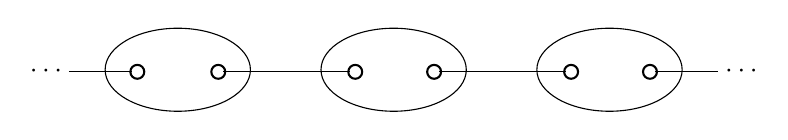
\begin{tikzpicture}[x=0.75pt,y=0.75pt,yscale=-1,xscale=1]
            %uncomment if require: \path (0,300); %set diagram left start at 0, and has height of 300
            
            %Straight Lines [id:da6245821686017994] 
            \draw    (108.5,125) -- (139.15,125) ;
            \draw [shift={(141.5,125)}, rotate = 0] [color={rgb, 255:red, 0; green, 0; blue, 0 }  ][line width=0.75]      (0, 0) circle [x radius= 3.35, y radius= 3.35]   ;
            %Straight Lines [id:da9728888558043336] 
            \draw    (182.85,125) -- (213.5,125) ;
            \draw [shift={(180.5,125)}, rotate = 0] [color={rgb, 255:red, 0; green, 0; blue, 0 }  ][line width=0.75]      (0, 0) circle [x radius= 3.35, y radius= 3.35]   ;
            %Shape: Ellipse [id:dp40247130481984605] 
            \draw   (126,124) .. controls (126,112.95) and (141.67,104) .. (161,104) .. controls (180.33,104) and (196,112.95) .. (196,124) .. controls (196,135.05) and (180.33,144) .. (161,144) .. controls (141.67,144) and (126,135.05) .. (126,124) -- cycle ;
            %Straight Lines [id:da5535258332135746] 
            \draw    (213.5,125) -- (244.15,125) ;
            \draw [shift={(246.5,125)}, rotate = 0] [color={rgb, 255:red, 0; green, 0; blue, 0 }  ][line width=0.75]      (0, 0) circle [x radius= 3.35, y radius= 3.35]   ;
            %Straight Lines [id:da2347934449839162] 
            \draw    (286.85,125) -- (317.5,125) ;
            \draw [shift={(284.5,125)}, rotate = 0] [color={rgb, 255:red, 0; green, 0; blue, 0 }  ][line width=0.75]      (0, 0) circle [x radius= 3.35, y radius= 3.35]   ;
            %Shape: Ellipse [id:dp5388082527929081] 
            \draw   (230,124) .. controls (230,112.95) and (245.67,104) .. (265,104) .. controls (284.33,104) and (300,112.95) .. (300,124) .. controls (300,135.05) and (284.33,144) .. (265,144) .. controls (245.67,144) and (230,135.05) .. (230,124) -- cycle ;
            %Straight Lines [id:da7687316396415951] 
            \draw    (317.5,125) -- (348.15,125) ;
            \draw [shift={(350.5,125)}, rotate = 0] [color={rgb, 255:red, 0; green, 0; blue, 0 }  ][line width=0.75]      (0, 0) circle [x radius= 3.35, y radius= 3.35]   ;
            %Straight Lines [id:da5902566541675356] 
            \draw    (390.85,125) -- (421.5,125) ;
            \draw [shift={(388.5,125)}, rotate = 0] [color={rgb, 255:red, 0; green, 0; blue, 0 }  ][line width=0.75]      (0, 0) circle [x radius= 3.35, y radius= 3.35]   ;
            %Shape: Ellipse [id:dp7785523629855451] 
            \draw   (334,124) .. controls (334,112.95) and (349.67,104) .. (369,104) .. controls (388.33,104) and (404,112.95) .. (404,124) .. controls (404,135.05) and (388.33,144) .. (369,144) .. controls (349.67,144) and (334,135.05) .. (334,124) -- cycle ;
            
            % Text Node
            \draw (106.5,125) node [anchor=east] [inner sep=0.75pt]    {$\cdots $};
            % Text Node
            \draw (423.5,125) node [anchor=west] [inner sep=0.75pt]    {$\cdots $};
            \end{tikzpicture}            
    \end{gathered} \eqqcolon \ket*{\Psi}.
\end{equation}